\documentclass[11pt,a4paper]{article}
\usepackage[left=2cm,text={17cm,25cm},top=2.5cm]{geometry}
\usepackage[T1]{fontenc}
\usepackage[english]{babel}
\usepackage[utf8]{inputenc}
\usepackage{url}
\usepackage{graphicx}
\usepackage{pdfpages}
\usepackage[colorinlistoftodos,prependcaption,textsize=tiny]{todonotes}

\graphicspath{ {figs/} }

\begin{document}

\begin{center}
	\LARGE{Soft Computing}\\
	\Large{Job Performance Evaluation Using Back-propagation Network}
	\vspace{0.5cm}

    \begin{centering}
    \small{
        Bc. Petr Stehlík <xstehl14@stud.fit.vutbr.cz>
        }
    \end{centering}

	\vspace{0.2cm}

\end{center}

\section{Assignment}
The aim of the project is to assemble a mechanical device and create software for acquiring 2D hand geometry using a line camera.
A solution for camera mount and hand placement is proposed in the following sections for best geometry acquisition and image reconstruction.

\section{Theoretical Background}
\label{sec:theory}

\subsection{Backpropagation Network}
Backpropagation networks are multi-layer feed-forward networks with supervised learning. There is no interconnection between neurons in the same layer but layers are fully connected to the next neighbouring layer in order to be able to do forward and backward propagation of values.

\subsubsection{Forward-propagation}
Each neuron in all layers but input layer disposes of a weight for each input initialized to a random value in range $<0,1>$, linear base function and sigmoidal activation function.

When forward propagating an input vector the vector is laid out onto the input neurons and the vector is recalculated using following formulas for the next layer until the input vector is propagated to the output layer which outputs the response of the whole network itself.

The base function is shown in equation \ref{eq:base}:

\begin{equation}
    f(\vec{x}) =\sum_{i = 0}^{n} w_i x_i
    \label{eq:base}
%    f(u) = \frac{1}{1 + e^{-\lambda u}}
\end{equation}

where $ \vec{x} $ is the input vector, $ w $ are weights for each input of given neuron and $ n $ is the length of the neuron input vector and bias (term used as in \cite{deeplearning}\cite{elements}) value resulting in $ n = |x| + 1$.

The sigmoidal activation function is presented in equation \ref{eq:act} where $ \lambda $ is a constant set to $ \lambda = 1 $ and in further equations left out because of this fact.

\begin{equation}
    g(u) = \frac{1}{1 + e^{-\lambda u}}
    \label{eq:act}
\end{equation}

The output of a neuron is then given by using the equations \ref{eq:base} and \ref{eq:act}:

\begin{equation}
    y = g( f( \vec{x} ) )
    \label{eq:output}
\end{equation}


\subsubsection{Back-propagation}
Back-propagation is used only when one trains the network and is one of the base methods for training feed-forward networks. The method is based on adjusting weights depending on the error calculated by equation \ref{eq:err} for an output neuron $ p $ using produced output ($ o $) and desired output ($ d $) values.

\begin{equation}
    E_p = \frac{1}{2} \sum_{j = 1}^{m} (d_{pj} - o_{pj})^2
    \label{eq:err}
\end{equation}

The change of weights is calculated using equation \ref{eq:delta} where $ \nabla E_p $ is the derived error gradient and $ \mu $ the learning rate.

\begin{equation}
    \Delta \vec{w_p} = -\mu \nabla E_p
    \label{eq:delta}
\end{equation}

To calculate one particular change of weight we use formula \ref{eq:neuron-delta} where $ L $ is the given layer of the network, $ j $ is the $j$-th neuron in layer $ L $ and $ i $ is the $i$-th input of the neuron $ j $.

\begin{equation}
    \Delta w_{ji}^L = \mu \delta_j^L x_i^L
    \label{eq:neuron-delta}
\end{equation}

For the output layer $ L $ of the network we use formula \ref{eq:output-err}.

\begin{equation}
    \delta_j^L = (d_j - y_j^L) y_j^L(1 - y_j^L)
    \label{eq:output-err}
\end{equation}

For hidden layers of the network, we use the same principle propagating the error backwards from the output layer as shown in equation \ref{eq:prop-err} where $\lambda = 1$ and therefore left out.

\begin{equation}
    \Delta {^l w}_{ji} = \mu {^l\delta}_j {^lx}_i = \mu \sum_{k = 1}^{n_{l+1}} (^{l+1}\delta_k {^{l+1}w}_{kj}) {^ly}_j (1 - ^ly_j){^lx}_i
    \label{eq:prop-err}
\end{equation}

Each repetition of forward and backward propagation of all inputs is called an epoch. Finally, we can choose when to update the weights, in batches after all input vectors were processed or using the stochastic method where weights are updated after processing each input vector.

\subsection{Examon}
\label{sec:examon}
Examon\cite{examon} framework is used for exascale monitoring of supercomputing facilities. It is built on top of MQTT protocol\cite{locke2010mqtt} which allows measured metrics to be sent to a central broker where received data are processed and stored in KairosDB\cite{KAIROS} database utilizing Cassandra\cite{CASSANDRA} cluster.

\begin{figure}[ht]
    \centering
    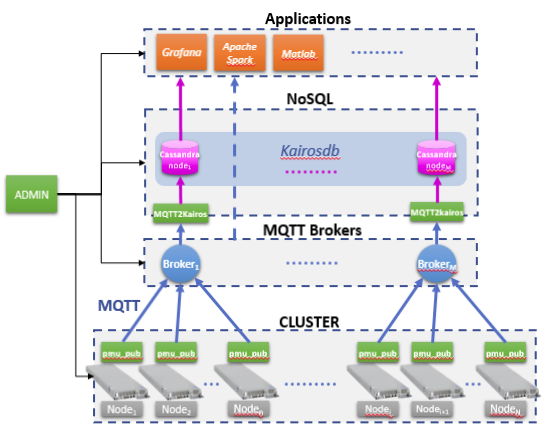
\includegraphics[width=0.45\linewidth]{examon-architecture}
    \caption{Examon framework architecture}
    \label{arch}
\end{figure}

KairosDB is used for storing metric data in time-series format whereas Cassandra, serving as a backend for KairosDB is also used for storing job-related data. More on data semantics is described~in~\ref{sec:data}.



\section{Data}
\label{sec:data}

As previously stated in \ref{sec:examon} data are gather via Examon framework and stored in Cassandra database. We can split the data into two categories. Job data and metric data.

The job data come from 


\section{Implementation}
In this section, we describe the implementation phase of the project. The project was implemented using Python 2.7.13. External library SciPy\cite{scipy} was used for linear data interpolation.

\label{sec:implementation}

\subsection{Data Acquisition}
\label{sec:data-filter}
First, job data were queried and filtered according to several rules:
\begin{itemize}
    \item job run time must be between 10 and 60 minutes
    \item job must occupy the whole node (multiplies of 16 cores)
    \item job must be run in 15-day period
\end{itemize}

This resulted in 32 jobs which gave enough diversity for correct classification. All datapoints were aggregated by 30 seconds using averaging aggregator available in KairosDB.

The rule of minimum 10 minutes is because of any shorter job is usually a development, not production version of a program and in current HPC facilities such program is very cheap to run and therefore no deep performance analysis is needed. The same goes for jobs smaller than one node (16 cores).

Jobs longer than one hour are not suited for training the network because of too large input vectors exceeding the scope of this project and the loss of information in further data processing.

\subsection{Data Labelling}
In order to correctly label all chosen jobs and their metrics a simple graphical user interface was made. The GUI is based on previous work done during the PRACE Summer of HPC called Examon Web which is an extension of Examon framework visualizing specific views of all collected data.

Visualization is done in timeseries fashion using Dygraphs library. This helps to better understand the correlations between all metrics and in time combined.

The GUI is shown in figure \ref{fig:ex-labeler} where you can see a check box for each metric and at the bottom a checkbox for the whole job. The metric checkbox labels the accompanying metric of suspicious behaviour and job one of suspicious behaviour of the job as a whole.

\begin{figure}[ht]
    \centering
    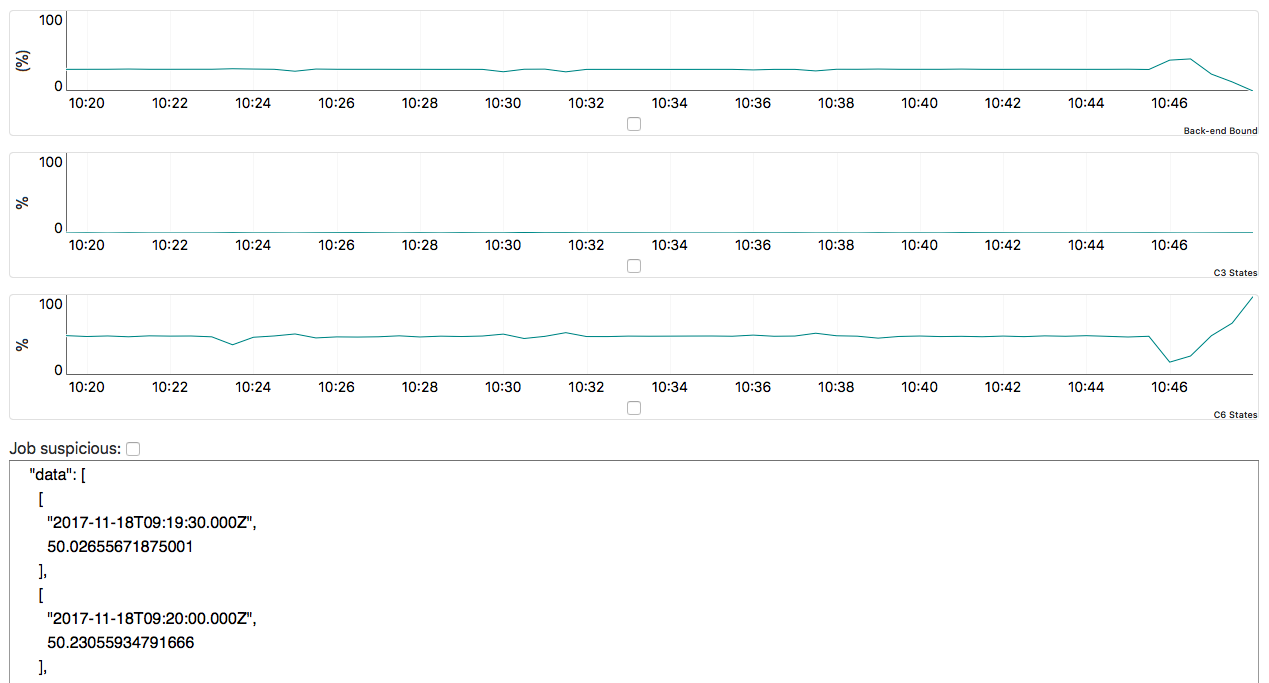
\includegraphics[width=0.75\linewidth]{examon-labeler}
    \caption{Part of Examon Web based data labelling tool}
    \label{fig:ex-labeler}
\end{figure}

\subsection{Data Processing}

After labelling the job all metric data with labels are generated and can be worked on further. All metric vectors were interpolated to 80 values which provides good performance/detail compromise. Larger input vectors resulted in extremely longer runs and smaller input vectors resulted in poor outputs of the network.

\subsection{Metric Networks}

To achieve best results/speed combination a backpropagation neural network was created for each metric. This gives us the total of twelve networks completely independent of each other which means the training process can be fully parallelized.

All metric networks were configured the same way to achieve uniform results. The input layer disposes of 80 neurons with hidden layers of 4 and then 3 neurons and one output neuron.

This configuration was chosen based on trial and error experiments.

\subsection{Job Network}
Once all metric networks compute their output we have a vector of 12 values which serves as an input to the job classification network.

The network is created with 12 input neurons, one hidden layer of 4 neurons and one output neuron.

All networks output a single value. Metric networks because of further processing in the job network and the job network because of clearer values.


\section{Achieved Results}
\label{sec:res}
Solution described in this report was assembled and implemented with excellent results. Integration of all hardware parts and software control results
in images being scanned quickly in resolution exceeding 60 MPx. During testing it was proved to be effective to not only scan images
of hand geometry but also fingerprints which leads to general purpose sensoric solution for capturing multiple biometric data. Furthermore,
the solution is able to function with very limited resources necessary and provides instant access to scanned images via a web serber. Complete scan of both of the subject's
hands can be done under 1 minute.

\section{Summary}
\label{sec:sum}

\end{document}
